\documentclass{article}
\usepackage{graphicx}

\setlength{\parindent}{0pt}

\begin{document}

\title{UADE 2.xx design specification}
\author{Heikki Orsila $<$heikki.orsila@iki.fi$>$}
\date{}
\maketitle

\section{Introduction}

\subsection{History}

UADE 1.xx was written to be a stand-alone program that had separate code
for each possible \emph{frontend} (\emph{user interface}), but there was
no internal structure to implement different frontends easily. By much
hacking some kind of pseudo-interface was created to facilitate following
frontends:
\begin{itemize}
  \item Beep Media Player
  \item MorphOS shell without interaction
  \item Unix shell without interaction
  \item Unix shell with small interaction
  \item XMMS plugin
\end{itemize}

It was a clear design problem that needed to be fixed. To force the separation
of frontend and \emph{uadecore} (emulator), UADE 2.xx removed all user
interface issues from the uadecore. Token-passing based messaging system was
implemented into the uadecore. A frontend would communicate with uadecore
through a token-passing based messaging protocol. The messaging protocol
has following commands:
\begin{description}
\item [Config] command is used to pass a file name of the emulation
configuration file. The file is named \emph{uaerc}.
\item [Score] command is used to pass file name of a binary run-time in M68k
machine language for the emulator. The binary run-time is called
\emph{score} or \emph{sound core}. The sound core contains implementations of
\emph{Eagleplayer} and \emph{AmigaOS} APIs.
\item [Player] command is used to pass a file name of a binary player plugin
in M68k machine language for the sound core. This is also called an
\emph{Eagleplayer plugin}.
\item [Module] command is used to pass a file name of a song to be played by
the associated Eagleplayer plugin.
\item [Read]
\item [Reboot]
\item [Set subsong]
\item [Ignore check]
\item [Song end not possible]
\item [Set ntsc]
\item [Filter]
\item [Set interpolation mode]
\item [Speed hack]
\item [Change subsong]
\item [Activate debugger]
\item [Token] command
\end{description}
Messages are answered by following replies:
\begin{description}
\item [MSG]
\item [Can't play]
\item [Can play]
\item [Song end]
\item [Subsong info]
\item [Player name]
\item [Module name]
\item [Format name]
\item [Data]
\end{description}.

\begin{figure}
\centering
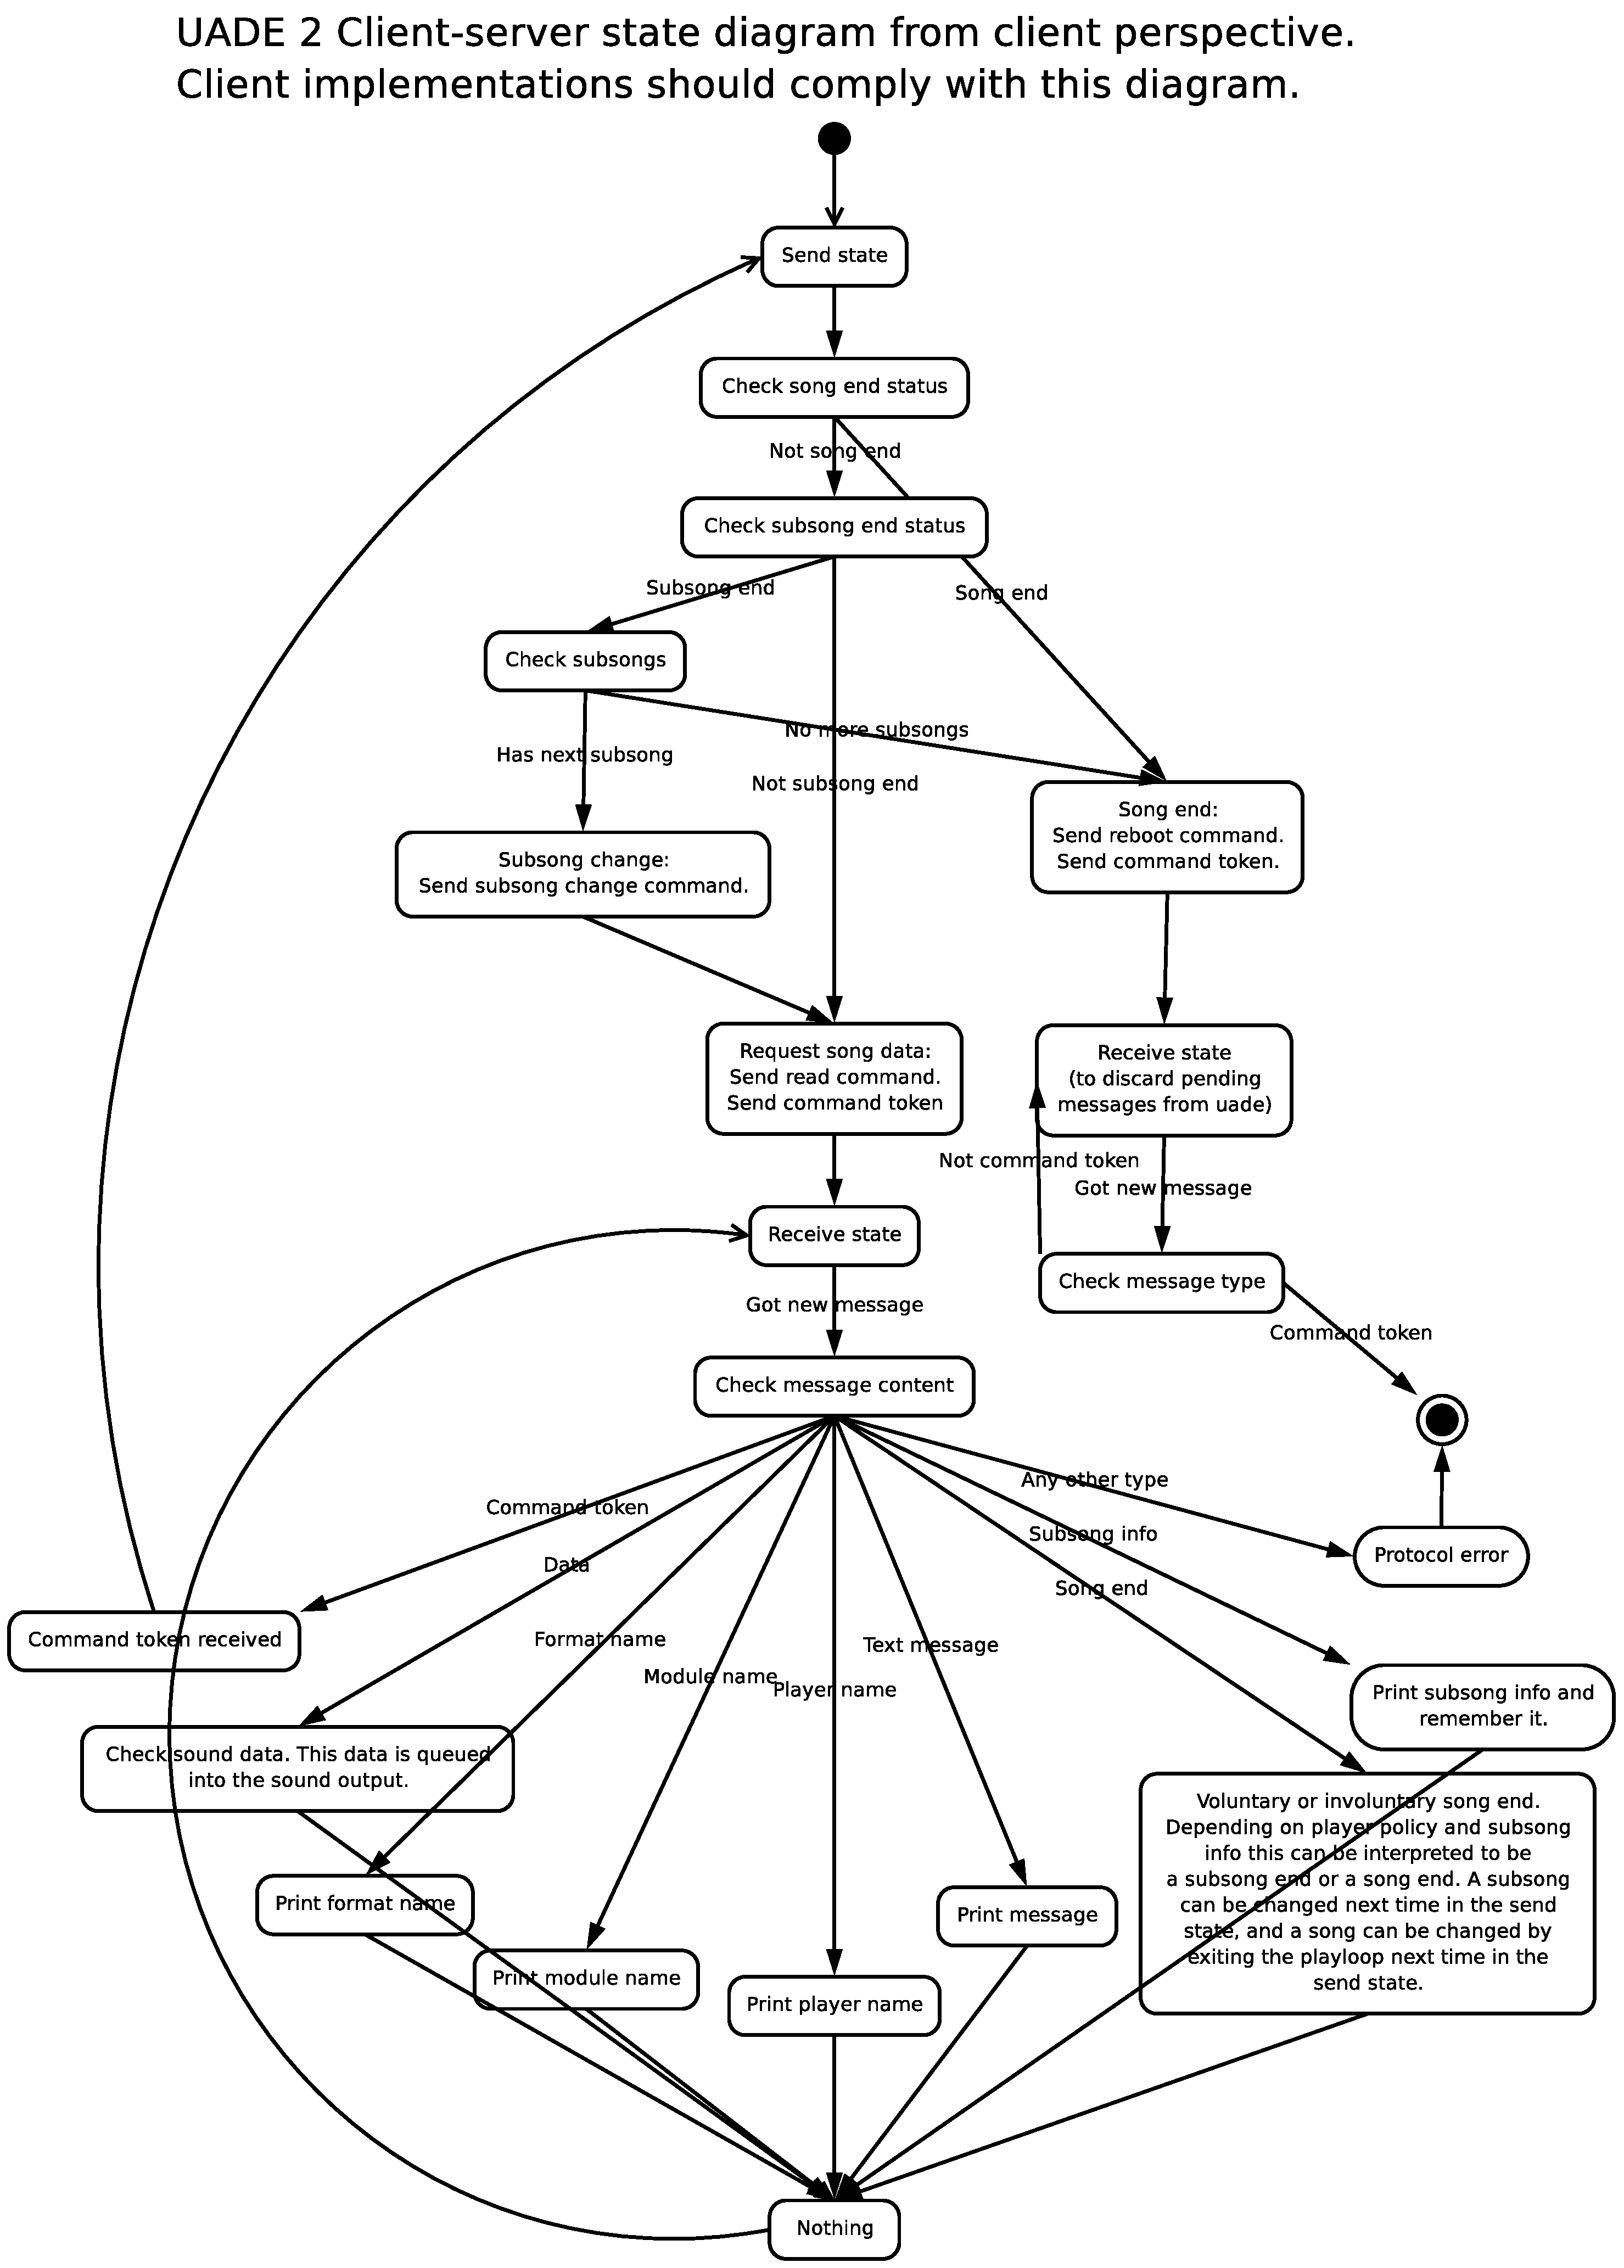
\includegraphics[scale=0.25]{play_loop_state_diagram.eps}
\caption{Play loop interaction from client (frontend) perspective}
\label{fig:playloop}
\end{figure}

\end{document}
